\documentclass{article}
\usepackage[margin=1in]{geometry}
\usepackage{problemset}
\showsolntrue

% Custom commands
\newcommand{\R}{\mathbb{R}}
\newcommand{\X}{\mathcal{X}}
\newcommand{\Y}{\mathcal{Y}}
\newcommand{\E}{\mathbb{E}}
\newcommand{\V}{\text{Var}}
\renewcommand{\P}{\mathbb{P}}

\begin{document}

\pstitle{%
    MATH 181A%
}{
    Homework 7%
}[due Thursday, Feb 26 at 11:59PM]

\begin{probset}
% --- Problem 1 ---
\begin{prob}[\textbf{6.3.9}]
    (Use exact binomial test) Suppose $H_0: p = 0.75$ is to be tested against $H_1: p < 0.75$ using a random sample of size $n = 7$ and the decision rule “Reject $H_0$ if $k \leq 3$.”

    \begin{subprobset}
    \begin{subprob}
        What is the test's level of significance?

        \begin{soln}
            The test's level of significance is given by $\P(k \leq 3)$ where $k \sim Binomial(7, 0.75)$. We find that $\P(k \leq 3) = \sum_{k=0}^{3} \binom{7}{k} (0.75)^k (0.25)^{7-k} \approx 0.0706$. So the test's level of significance is 0.0706.
        \end{soln}
    \end{subprob}

    \begin{subprob}
        Compute the power of the test when $p = 0.65$.

        \begin{soln}
            The power of the test when $p = 0.65$ is given by $\P(k \leq 3)$ where $k \sim Binomial(7, 0.65)$. We find that $\P(k \leq 3) = \sum_{k=0}^{3} \binom{7}{k} (0.65)^k (0.35)^{7-k} \approx 0.1998$. So the power of the test when $p = 0.65$ is 0.1998.
        \end{soln}
    \end{subprob}
    \end{subprobset}
\end{prob}

% --- Problem 2 ---
\begin{prob}
    You should first do question 6.2.2 with $z_{\alpha/2} = 1.88$ for $\alpha = 0.06$.

    \begin{subprobset}
    \begin{subprob}
        (\textbf{6.2.2}) An herbalist is experimenting with juices extracted from berries and roots that may have the ability to affect the Stanford-Binet IQ scores of students afflicted with mild cases of attention deficit disorder (ADD). A random sample of twenty-two children diagnosed with the condition have been drinking Berry Smart daily for two months. Past experience suggests that children with ADD score an average of 95 on the IQ test with a standard deviation of 15. If the data are to be analyzed using the $\alpha = 0.06$ level of significance, what values of $y$ would cause $H_0$ to be rejected? Assume that $H_1$ is two-sided.

        \begin{soln}
            The critical values are found from the 3rd and 97th quantiles of $Normal(95, 15/\sqrt{22}) = [88.99, 101.01]$. So the critical region is $y \leq 88.99$ or $y \geq 101.01$.
        \end{soln}
    \end{subprob}

    \begin{subprob}
        (\textbf{6.4.3}) For the decision rule found in \textbf{6.2.2} to test $H_0: \mu = 95$ versus $H_1: \mu \neq 95$ at the $\alpha = 0.06$ level of significance, calculate $1 - \beta$ when $\mu = 90$.

        \begin{soln}
            The power is $\P(y \leq 88.99) + \P(y \geq 101.01)$ where $y \sim Normal(90, 15/\sqrt{22})$. We find that $\P(y \leq 88.99) + \P(y \geq 101.01) \approx 0.376$. So $1 - \beta$ is about 0.376.
        \end{soln}
    \end{subprob}
    \end{subprobset}
\end{prob}

\newpage

% --- Problem 3 ---
\begin{prob}[\textbf{6.4.7}]
    If $H_0: \mu = 200$ is to be tested against $H_1: \mu < 200$ at the $\alpha = 0.10$ level of significance based on a random sample of size $n$ from a normal distribution where $\sigma = 15.0$, what is the smallest value for $n$ that will make the power equal to at least 0.75 when $\mu = 197$?

\begin{verbatim}
from scipy import stats

z = stats.norm.ppf(0.10)
se = lambda n: 15 / (n ** 0.5)

for n in range(1, 100):
    c = 200 + z * se(n)
    power = stats.norm.cdf((c - 197) / se(n))
    if power >= 0.75:
        print(f"{n=}: {power=:.4f}")
        break
\end{verbatim}

    \begin{soln}
        Running the code above, we find that the smallest value for $n$ that will make the power equal to at least 0.75 when $\mu = 197$ is $n = 96$.
    \end{soln}
\end{prob}

% --- Problem 4 ---
\begin{prob}[\textbf{6.4.14}]
    A sample of size 1 is taken from the pdf 
    \[
        f_Y(y) = (\theta + 1)y^\theta, 0 \leq y \leq 1
    \]
    The hypothesis $H_0: \theta = 1$ is to be rejected in favor of $H_1: \theta > 1$ if $y \geq 0.90$. What is the test's level of significance?

    \begin{soln}
        The test's level of significance is given by $\P(y \geq 0.90)$ where $y \sim f_Y(y) = 2y$. We find that $\P(y \geq 0.90) = \int_{0.90}^1 2y dy = 1 - 0.9^2 = 0.19$. So the test's level of significance is 0.19.
    \end{soln}
\end{prob}

% --- Problem 5 ---
\begin{prob}[\textbf{6.4.20}]
    Suppose that one observation from the exponential pdf, $f_Y(y) = \lambda e^{-\lambda y}, y > 0$, is to be used to test $H_0: \lambda = 1$ versus $H_1: \lambda < 1$. The decision rule calls for the null hypothesis to be rejected if $y \geq \ln 10$. Find $\beta$ as a function of $\lambda$.

    \begin{soln}
        This can be found by integrating the pdf of $H_1$ from 0 to $\ln 10$.
        \[
            \beta = \int_{0}^{\ln 10} \lambda e^{-\lambda y} dy = \left[ -e^{-\lambda y} \right]_{0}^{\ln 10} = 1 - e^{-\lambda \ln 10} = 1 - 10^{-\lambda}
        \]
    \end{soln}
\end{prob}

\newpage

% --- Problem 6 ---
\begin{prob}[\textbf{6.4.24}]
    Given the pdf $f_Y(y; \theta) = 2y/\theta^2, 0 \leq y \leq \theta$. Take a sample of size 3 from this pdf. Use the statistic $Y_{\max}$ to test $H_0: \theta = 5$ versus $H_1: \theta > 5$. Recall that for $n = 3$ the pdf of $Y_{\max}$ is $f_{Y_{\max}}(y; \theta) = 6y^5/\theta^6, 0 \leq y \leq \theta$.

    \begin{subprobset}
    \begin{subprob}
        Find the critical value to give a test of significance $\alpha = 0.05$.

        \begin{soln}
            The critical value is found from the 95th quantile of $f_{Y_{\max}}(y; 5) = 6y^5/5^6$, i.e. where
            \[
                0.95 = \int_0^c \frac{6y^5}{5^6} dy = \frac{6}{5^6} \int_0^c y^5 dy = \frac{6}{5^6} \left[\frac{y^6}{6}\right]_0^c = \frac{c^6}{5^6} \implies c = 5\sqrt[6]{0.95} \approx 4.957
            \]
        \end{soln}
    \end{subprob}

    \begin{subprob}
        Suppose $\theta = 7$. What is the probability of Type II error for the test in part (a).

        \begin{soln}
            We can find $\beta$ by integrating the pdf of $H_1$ from the critical value to $\theta$.
            \[
                \beta = \int_{0}^{5\sqrt[6]{0.95}} \frac{6y^5}{7^6} dy = \frac{6}{7^6} \int_{0}^{5\sqrt[6]{0.95}} y^5 dy = \frac{6}{7^6} \left[\frac{y^6}{6}\right]_{0}^{5\sqrt[6]{0.95}} = \frac{5^6 \cdot 0.95}{7^6} \approx 0.126
            \]
        \end{soln}
    \end{subprob}
    \end{subprobset}
\end{prob}

\newpage

% --- Problem 7 ---
\begin{prob}[\textbf{R Simulation}]
    Let $X_1, \ldots, X_n$ be a random sample from $N (\mu, \sigma^2)$. Test $H_0: \mu = \mu_0$ against $H_1: \mu \neq \mu_0$. Define the effect size $\delta = \frac{\mu - \mu_0}{\sigma}$, the number of standard deviations the true mean is away from the tested one.

    \begin{subprobset}
    \begin{subprob}
        If it is known that $\sigma^2 = 1$, given $\alpha = 0.05$, derive a formula which shows how the power depends on the effect size $\delta$ and sample size $n$. You can use the notation $\Phi(x)$ to indicate the cumulative distribution function of the standard normal distribution.

        \begin{soln}
            With $\sigma^2 = 1$, we reject $H_0$ when $\frac{|\bar{X} - \mu_0|}{\sigma/\sqrt{n}} = \sqrt{n}|\bar{X} - \mu_0| > z_{\alpha/2} = 1.96$. 
            
            Under $H_1$, $\bar{X} \sim N(\mu, 1/n)$, so $\E[Z] = \E[\sqrt{n}(\bar{X} - \mu_0)] = \sqrt{n}(\mu - \mu_0)$ and $\V[Z] = \V[\sqrt{n}(\bar{X} - \mu_0)] = n\frac{1}{n} = 1$. Thus, under $H_1$, $Z \sim N(\sqrt{n}(\mu - \mu_0), 1)$. With $\delta = (\mu - \mu_0)/\sigma = \mu - \mu_0$, we have $Z \sim N(\delta\sqrt{n}, 1)$ under $H_1$. Thus
            \[
                \text{Power} = \P\left(|\sqrt{n}(\bar{X} - \mu_0)| > 1.96\right) = \Phi(-1.96 - \delta\sqrt{n}) + 1 - \Phi(1.96 - \delta\sqrt{n}).
            \]
        \end{soln}
    \end{subprob}

    \begin{subprob}
        Plot $\delta$ (x-axis with range [-2, 2]) versus power (y-axis) for $n = 10$ and $40$ in one figure. Comment on how the power changes with $\delta$ and $n$ from the plot.

        \begin{verbatim}
delta <- seq(-2, 2, length.out = 200)
power_n10 <- pnorm(-1.96 - sqrt(10) * delta) + 1 - pnorm(1.96 - sqrt(10) * delta)
power_n40 <- pnorm(-1.96 - sqrt(40) * delta) + 1 - pnorm(1.96 - sqrt(40) * delta)

par(pin = c(8, 5))
plot(delta, power_n10, type = "l", col = "blue", lwd = 2,
        xlab = expression(delta), ylab = "Power",
        main = "Power vs Effect Size (two-sided test, alpha = 0.05)",
        ylim = c(0, 1))
lines(delta, power_n40, col = "red", lwd = 2)
legend("bottomright", legend = c("n = 10", "n = 40"),
        col = c("blue", "red"), lty = 1, lwd = 2)
abline(h = 0.05, lty = 2, col = "gray")
        \end{verbatim}

        \begin{soln}
            \begin{center}
                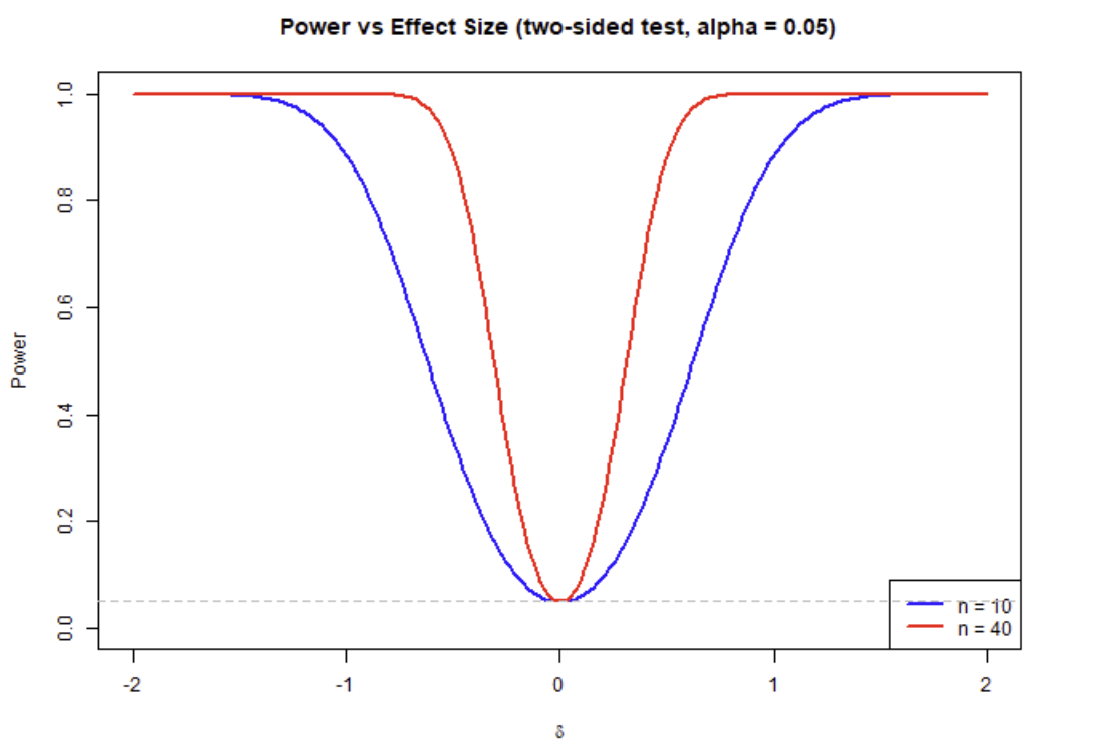
\includegraphics[width=0.6\textwidth]{Images/7b.png}
            \end{center}
            The power increases as $|\delta|$ increases. For a given power, a larger sample size allows a smaller $|\delta|$ to achieve it. The power is also symmetric around $\delta = 0$ which is expected since the test is two-sided. At its lowest, the power approaches $\alpha = 0.05$ as the effect size disappears.
        \end{soln}
    \end{subprob}
    \end{subprobset}
\end{prob}
\end{probset}
\end{document}